\documentclass[10pt]{beamer}
\usepackage{fancyvrb}
\usepackage{times}
\usepackage{pgf,pgfarrows,pgfnodes,pgfautomata,pgfheaps}
\usepackage{amsmath,amssymb}
\usepackage[utf8]{inputenc}
\usepackage{colortbl}
\usepackage[portuges]{babel}
\usepackage{graphicx}
\usepackage{color}
\usepackage{hyperref}
\usepackage{pxfonts,txfonts}
\usepackage{url}
\usepackage{underscore}
\usepackage[T1]{fontenc}

\usefonttheme{structurebold}
%insert for WSCAD19
\usepackage{multirow}
\usepackage{subfigure}
\usepackage{multicol}
\usepackage{adjustbox}
\usepackage{scalefnt}
%==================================================================================
\definecolor{DarkGreen}{rgb}{0,.5,0}
\definecolor{DarkRed}{rgb}{.5,0,0}
\definecolor{DarkBlue}{rgb}{0,0,.5}

\newcommand{\x}{\textbf{\textcolor{DarkGreen}{$\surd$}}}
\newcommand{\xx}{\textbf{\textcolor{DarkBlue}{$\odot$}}}
\newcommand{\xxx}{\textbf{\textcolor{DarkRed}{$\times$}}}
%==================================================================================

\usepackage{listings}
\renewcommand{\lstlistingname}{Programa}

\lstset{
numbers=left,
stepnumber=1,
firstnumber=1,
numberstyle=\tiny,
extendedchars=true,
breaklines=true,
frame=tb,
basicstyle=\footnotesize,
stringstyle=\ttfamily,
showstringspaces=false
}

%==================================================================================

\usetheme{Amsterdam}

%==================================================================================

\usecolortheme{default}
\setbeamertemplate{navigation symbols}{}

% inserir logotipo na apresentação
\pgfdeclareimage[height=0.5cm]{logo}{img/lups_oficial.png}
\logo{\pgfuseimage{logo}}
%Tinha a logo de outros orgãos 
\setbeameroption{hide notes}
%==================================================================================

\title[]{Estudo de viabilidade do uso de Raspberry PI na névoa}
\author[]{\textbf{\underline{Guilherme de Souza}\\ Nelson Lago \\ Prof. Dr. Gerson Cavalheiro\\ Prof. Dr. Alfredo Goldman\\}
Centro de Desenvolvimento Tecnológico\\
Bolsista PROBIC/PROBITI\\
 WSCAD 2019\\
 gdsdsilva@inf.ufpel.edu.br\\
}

\date{Outubro -- 2019  -- Campo Grande/MS}

%==================================================================================

\begin{document}
\frame[label=titlepage]{\titlepage \vspace{-1cm} \hspace{-1cm}}


\section{Introdução}
\frame{
    \frametitle{Introdução}
    \begin{block}{\textbf{Introdução}}
    \begin{itemize}
      \item Com o aumento de dispositivos que produzem e/ou consomem dados, maior tornou-se a demanda de processamento. Como resposta, rescursos disponiveis na nuvem foram empregados.
      \item O processamento pode ocorrer em \textit{data centers} geograficamente distantes, assim aplicações que dependem de uma baixa latência tendem a sofrer com o caminho percorrido até a nuvem.
      \item Com isso, um novo paradigma foi proposto, a \emph{Computação em Névoa}, que estende a Computação em Nuvem.
    \end{itemize}
  \end{block}
}

%% ---
\frame{
    \frametitle{Computação em Névoa}
    \begin{figure}[!tbp]
      \centering
      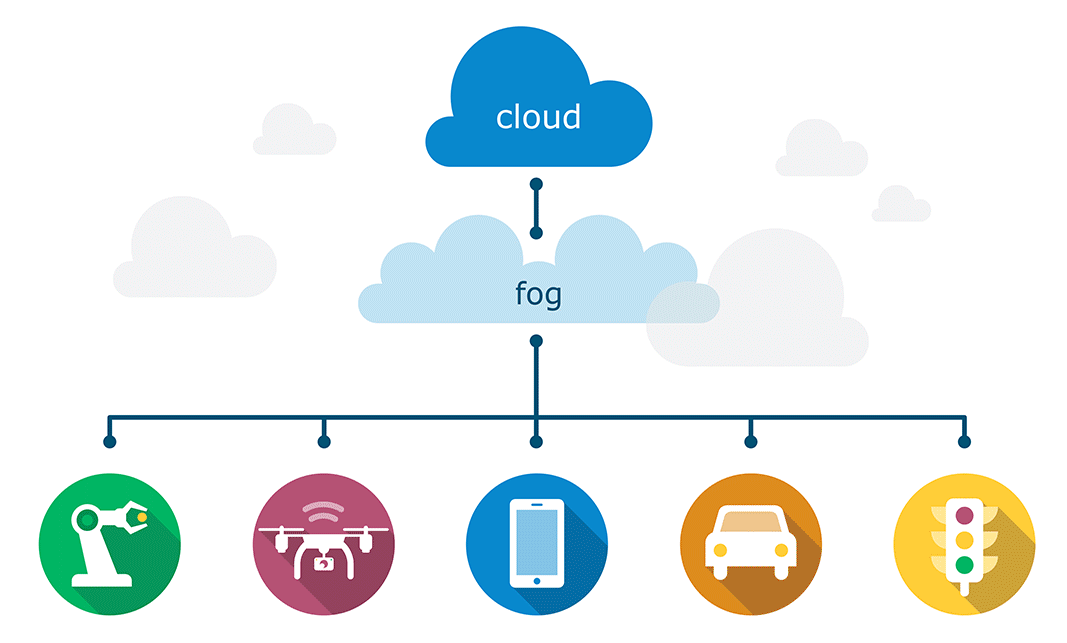
\includegraphics[width=0.80\textwidth]{img/imageFog.png}\label{fig:f1}
    \end{figure}
}
%% ---

\frame{
  \frametitle{Introdução}
  \begin{block}{Questionamento Central}
    \begin{figure}[!tbp]
      \centering
      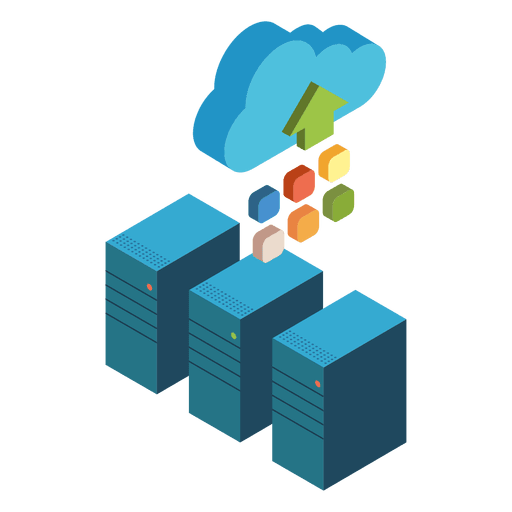
\includegraphics[width=0.25\textwidth]{img/nuvem.png}\label{fig:f1}
    \end{figure}
    \centering{\normalsize \bf \textit{Hardwares} de baixo consumo energético como parte de uma Névoa computacional são viáveis?}
  \end{block}
}
\frame{
  \frametitle{Objetivos}
  \begin{block}{Gerais}
    \begin{itemize}
      \item Quantativar a capacidade computacional de \textit{hardwares} de baixo consumo utilizando um \textit{benchmark}.  
    \end{itemize}
  \end{block}
  \begin{block}{Específicos}
    \begin{itemize}
      \item Definir o \textit{benchmark} que melhor atende aos objetivos do trabalho; 
      \item Decidir qual \textit{hardware} é o adequado para suprir as necessidades propóstas.
    \end{itemize}
  \end{block}
}
%% ---

%==================================================================================
\section{Metodologia}
\frame{
    \frametitle{Metodologia}
    \begin{block}{\textit{Especificações}}
        \begin{table}[]
            \begin{tabular}{c|c}
                \textbf{Especificação} & \textbf{Raspberry PI 3}                                                  \\ \hline
                Processador            & \begin{tabular}[c]{@{}c@{}}BCM2837 64Bit\\ QUAD Core 1.2GHz\end{tabular} \\ \hline
                    Arquitetura            & ARMv8                                                                    \\ \hline
                    RAM                    & 1GB SDRAM 400MHz                                                         \\ \hline
                    Armazenamento          & MicroSD                                                                  \\ \hline
                    Corrente / Tensão      & 1,34A / 5V                                                               \\ \hline
            \end{tabular}
        \end{table}
    \end{block}
}

\frame{
  \frametitle{Metodologia}
  \begin{block}{Banco de Dados}
      \begin{itemize}
          \item Visto que a demanda de serviços \textit{web} ocupa a maior parte das aplicações na nuvem, para a realização deste trabalho optou-se pelo uso de um banco de dados NoSQL.
              \begin{itemize}
                      \item Apache Cassandra.
              \end{itemize}
      \end{itemize}
  \end{block}
}

\frame{
    \frametitle{Metodologia}
    \begin{block}{Benchmark}
        \begin{itemize}
          \item O \textit{benchmark} escolhido foi o \textit{Netflix Data Benchmark}~(\textbf{NDBench}):
          \begin{itemize}
            \item Mede o desempenho de uma aplicação de banco de dados no dispositivo escolhido;
            \item Obtem informações como, operações na memória cache e resultados de latência em percentil.
          \end{itemize}
        \end{itemize}
    \end{block}
}

\frame{
    \frametitle{Metodologia}
    \begin{block}{Principais propriedades das cargas}
        \begin{table}[]
            \scalefont{0.98}
            \begin{adjustbox}{scale=0.815}
                \begin{tabular}{c|c}
                    \textbf{Config. Nome}                                                    & \textbf{Descrição}                                                                                                           \\ \hline
                    numKeys                                                                  & Espaço amostral para as chaves geradas aleatoriamente                                                                        \\ \hline
                    numValues                                                                & Espaço amostral para os valores gerados                                                                                      \\ \hline
                    dataSize                                                                 & Tamanho de cada valor                                                                                                        \\ \hline
                    \begin{tabular}[c]{@{}c@{}}numWrites /\\ numReaders\end{tabular}         & \begin{tabular}[c]{@{}c@{}}Número de threads por nodo NDBench para\\ gravações / leituras\end{tabular}                       \\ \hline
                        \begin{tabular}[c]{@{}c@{}}writeEnabled /\\ readEnabled\end{tabular}     & Booleano para ativar ou desativar escrita ou leitura                                                                         \\ \hline
                            \begin{tabular}[c]{@{}c@{}}writeRateLimit /\\ readRateLimit\end{tabular} & Número de gravações e leituras por segundo                                                                                   \\ \hline
                                userVariableDataSize                                                     & \begin{tabular}[c]{@{}c@{}}Booleano para ativar / desativar a capacidade da\\ carga a ser gerada aleatóriamente\end{tabular} \\ \hline
                \end{tabular}
            \end{adjustbox}
        \end{table}
    \end{block}
}

\frame{
    \frametitle{Metodologia}
    \begin{block}{Parâmetros de entrada}
    \begin{table}[!ht]
        \centering
        %\caption{Valores atribuídos às variáveis de execução do \textit{NDBench} durante os diferentes experimentos executados.}
        \begin{tabular}{c|ccc}
            \multirow{2}{*}{\textbf{Parâmetro}} & \multicolumn{3}{c}{\textbf{Valores atribuídos}}                                                                    \\ \cline{2-4} 
            & \multicolumn{1}{c|}{\textbf{Experimento 1}} & \multicolumn{1}{c|}{\textbf{Experimento 2}} & \textbf{Experimento 3} \\ \hline
            numWrite                            & \multicolumn{1}{c|}{256 Threads}            & \multicolumn{1}{c|}{256 Threads}            & 256 Threads            \\ \hline
            numRead                             & \multicolumn{1}{c|}{256 Threads}            & \multicolumn{1}{c|}{256 Threads}            & 256 Threads            \\ \hline
            writeRateLimit                      & \multicolumn{1}{c|}{2.000 e/s}              & \multicolumn{1}{c|}{0 e/s}                  & 500 e/s                \\ \hline
            readRateLimit                       & \multicolumn{1}{c|}{0 l/s}                  & \multicolumn{1}{c|}{2.000 l/s}              & 1.500 l/s              \\ \hline
        \end{tabular}
    \end{table} 
    \end{block}
    }

    \frame{
        \frametitle{Metodologia}
        \begin{block}{Metodologia do teste}
            \begin{itemize}
                \item Seguindo a documentação de ambas ferramentas "levantou-se" ambos ambientes para execução dos experimentos;
                    %e utilizando um script de execução, que realizava os seguintes passos para cada \textit{workload}:
                \item Para execução do \textit{NDBench} criou-se \textit{scripts} python, tanto para automatização, quanto para precisão de inicio e fim dos experimentos;
                \item Os \textit{scripts} ajustavam os parâmetros de entrada de acordo com a tabela apresentada e, executava durante 25 minutos.
            \end{itemize}
        \end{block}
    }

\frame{
  \frametitle{Metodologia}
    \begin{figure}[!ht]
        \centering
        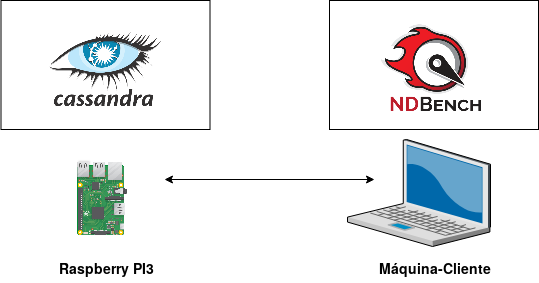
\includegraphics[scale=0.5]{img/ambienteExecucao.png}
        \label{fig:ambiente}
    \end{figure}
}

%==================================================================

\section{Resultados}
\frame{
    \frametitle{Resultados}
    \begin{block}{Total de sucesso e falhas}
        \begin{table}[!hb]
            \centering
           % \caption{Total de escritas e leituras alcançadas com sucesso e falhas ao final de 25 minutos. \label{tab:result_in_table}}
            \begin{tabular}{c|c|c|cc}
                \multirow{2}{*}{\textbf{Experimentos}} & \multicolumn{2}{c|}{\textbf{Escrita}} & \multicolumn{2}{c}{\textbf{Leitura}}                   \\ \cline{2-5} 
                & \textbf{Sucesso}   & \textbf{Falha}   & \multicolumn{1}{c|}{\textbf{Sucesso}} & \textbf{Falha} \\ \hline
                Experimento 1                         & 1.990.963          & 2.585            & \multicolumn{1}{c|}{-}                & -              \\ \hline
                Experimento 2                         & -                  & -                & \multicolumn{1}{c|}{2.155.112}        & 0              \\ \hline
                Experimento 3                         & 834.606            & 26               & \multicolumn{1}{c|}{808.983}          & 0              \\ \hline
            \end{tabular}
        \end{table}
    \end{block}
}

\frame{
    \frametitle{Experimento 1}
    \framesubtitle{Latência de escrita}
    \begin{figure}[!ht]
        \centering
        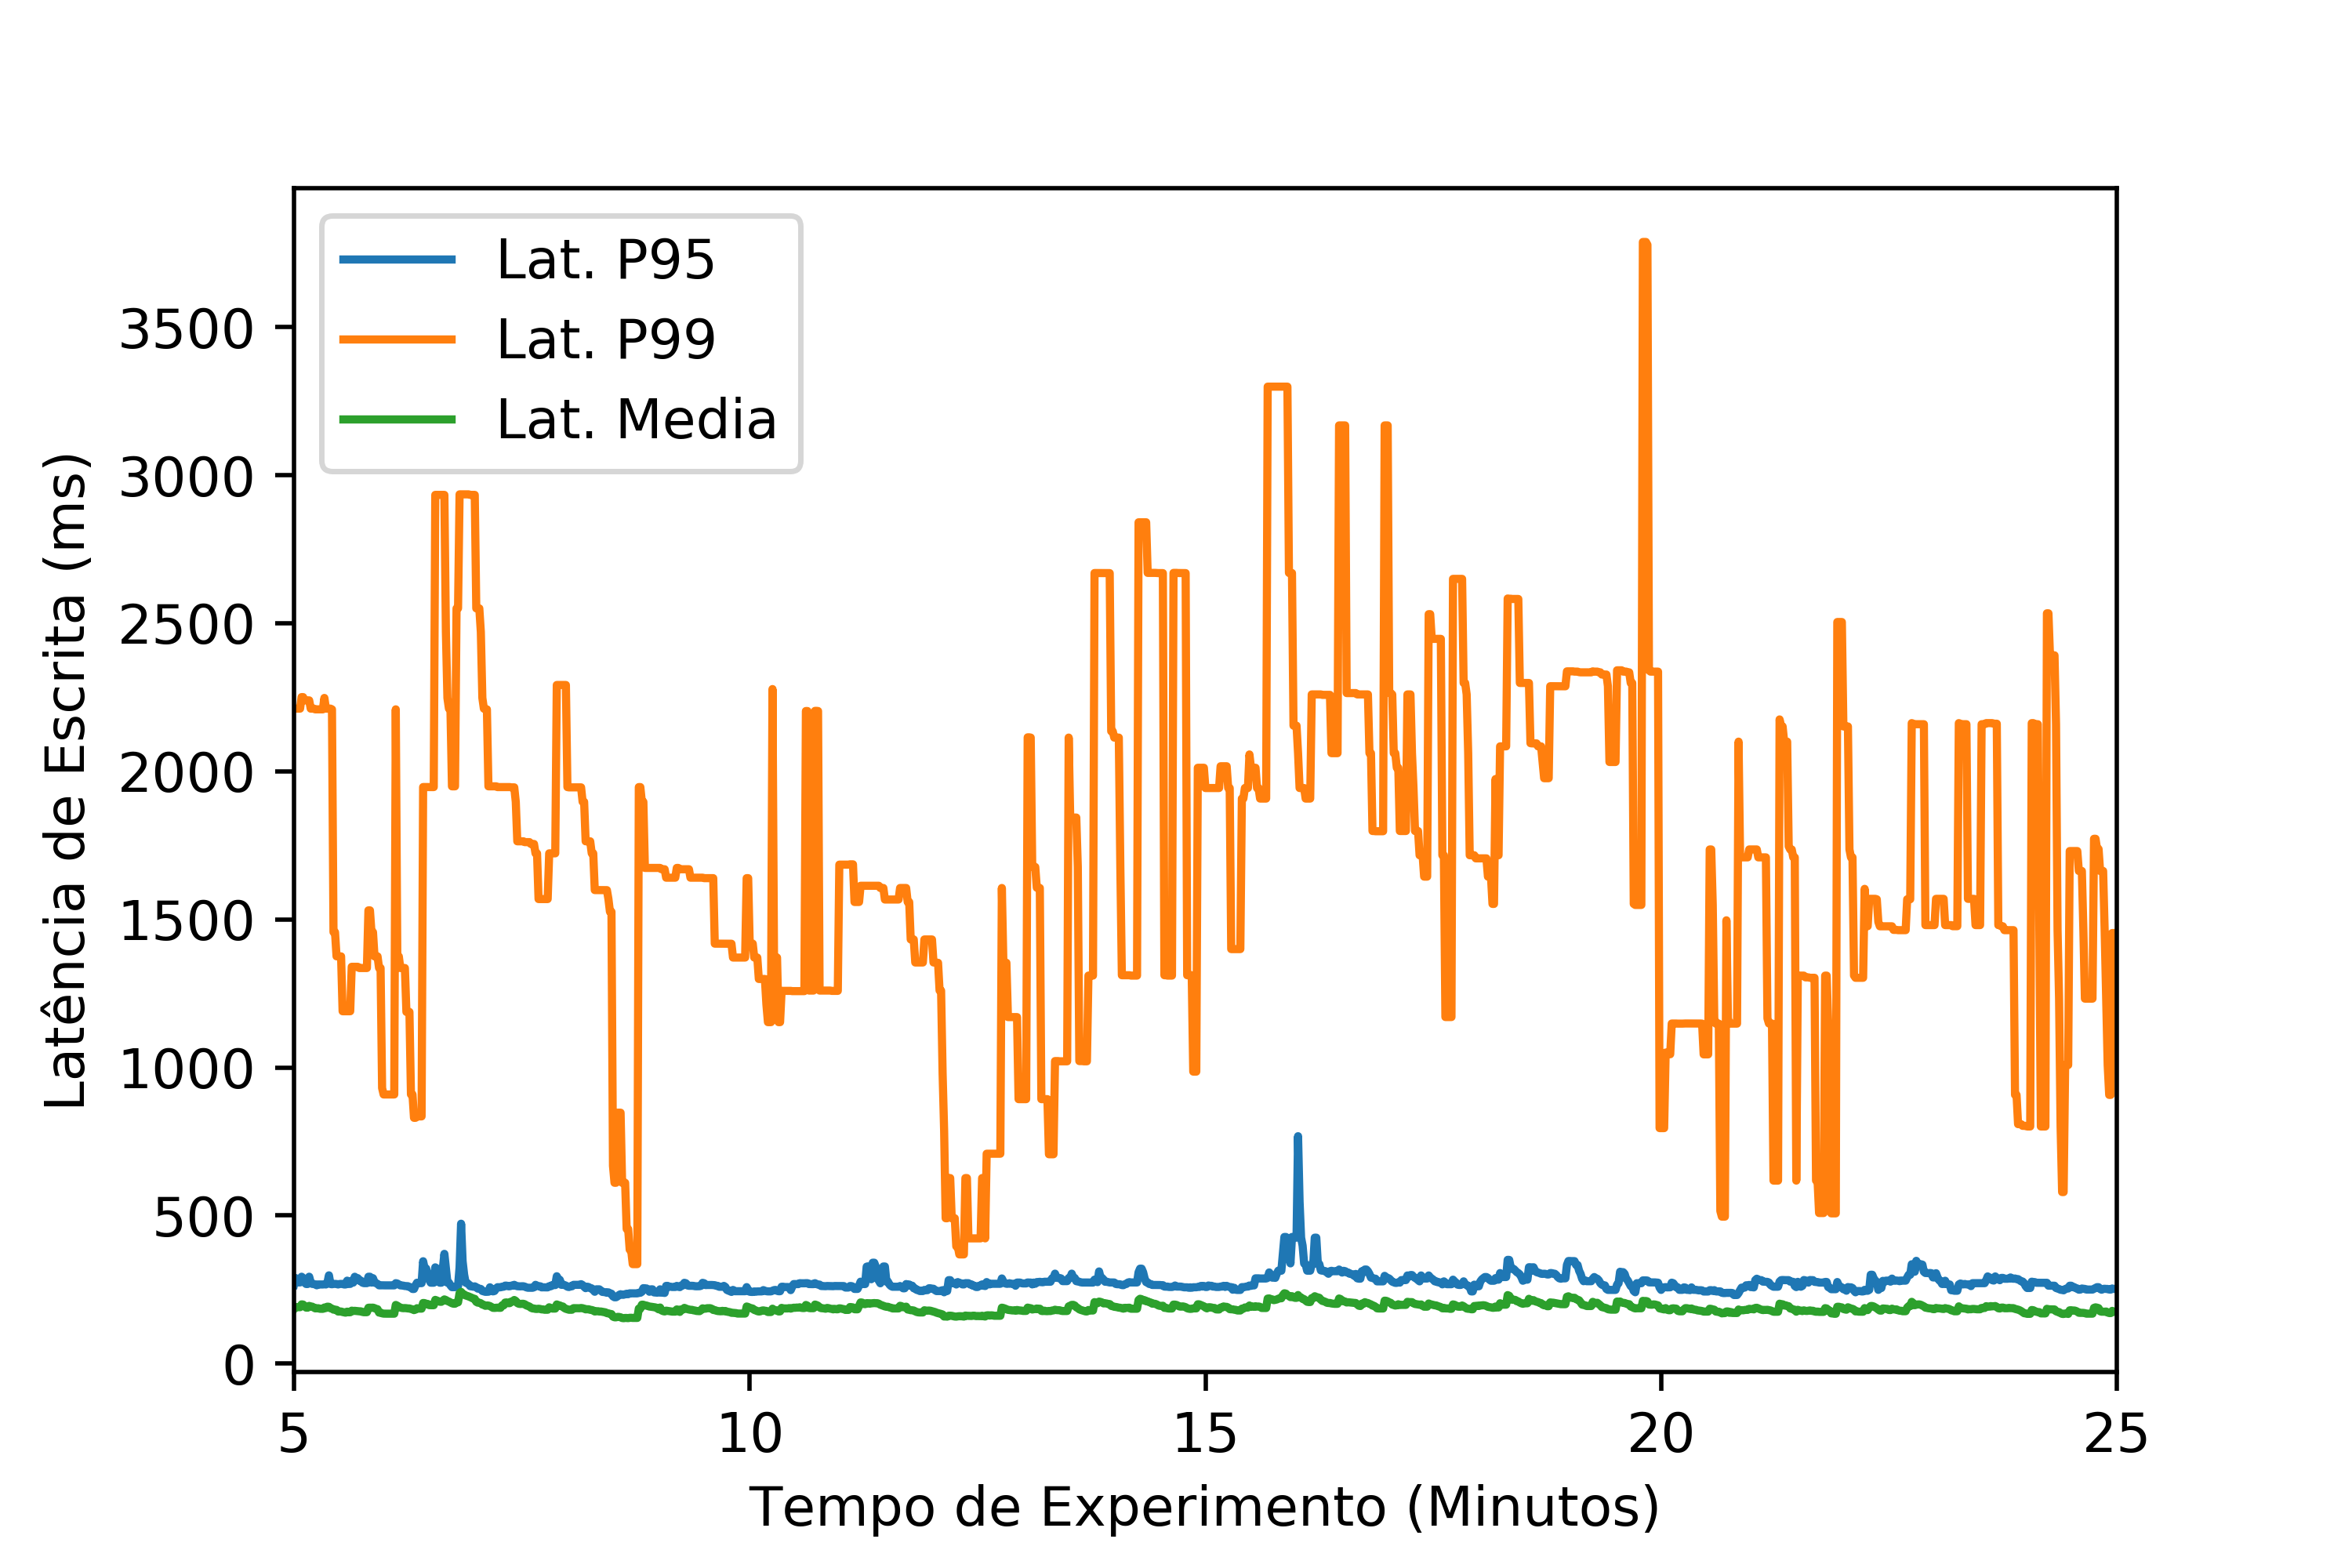
\includegraphics[scale=0.5]{img/pi3Write.png}
        \caption{Latências por segundo durante escrita no período de execução de 25m desconsiderando os 5m iniciais do simulador.}
        \label{fig:write}
    \end{figure}
}

\frame{
    \frametitle{Experimento 1}
    \framesubtitle{RPS de escrita}
    \begin{figure}[!ht]
        \centering
        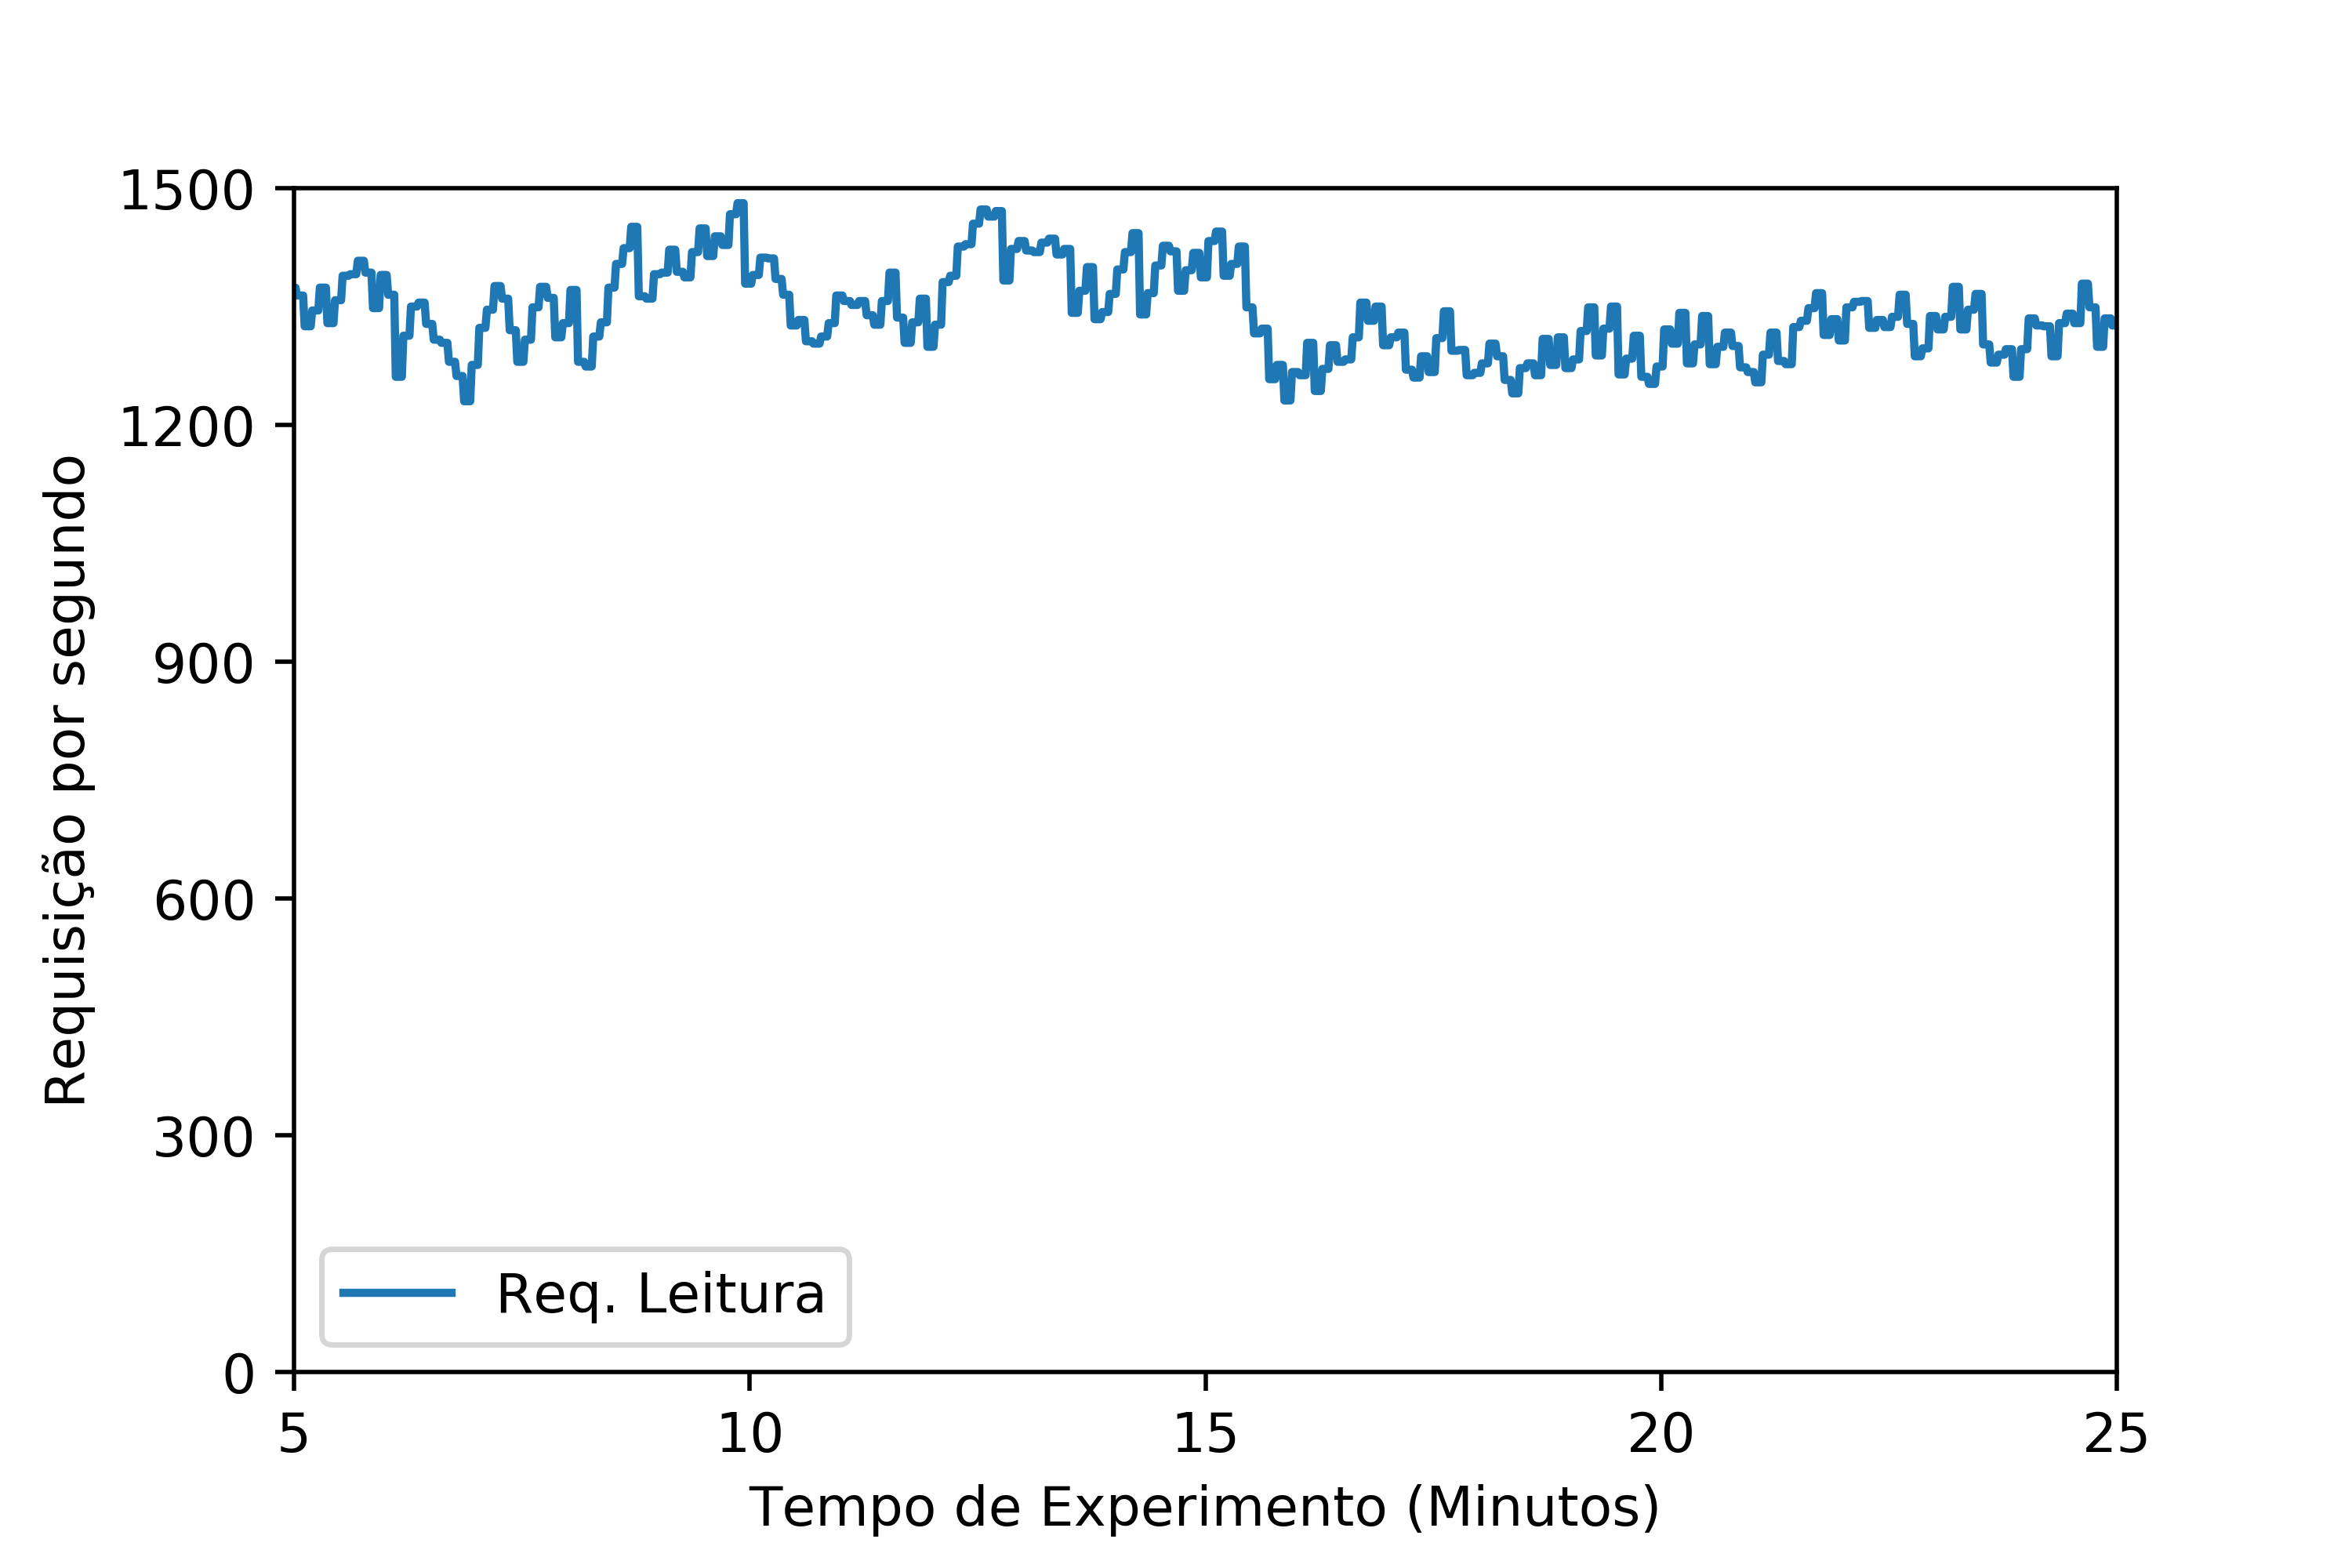
\includegraphics[scale=0.5]{img/pi3WriteRPS.png}
        \caption{Requisições por segundo durante escrita no período de execução de 25m desconsiderando os 5m iniciais do simulador.}
        \label{fig:writeRPS}
    \end{figure}
}

\frame{
    \frametitle{Experimento 2}
    \framesubtitle{Latência de leitura}
    \begin{figure}[!ht]
        \centering
        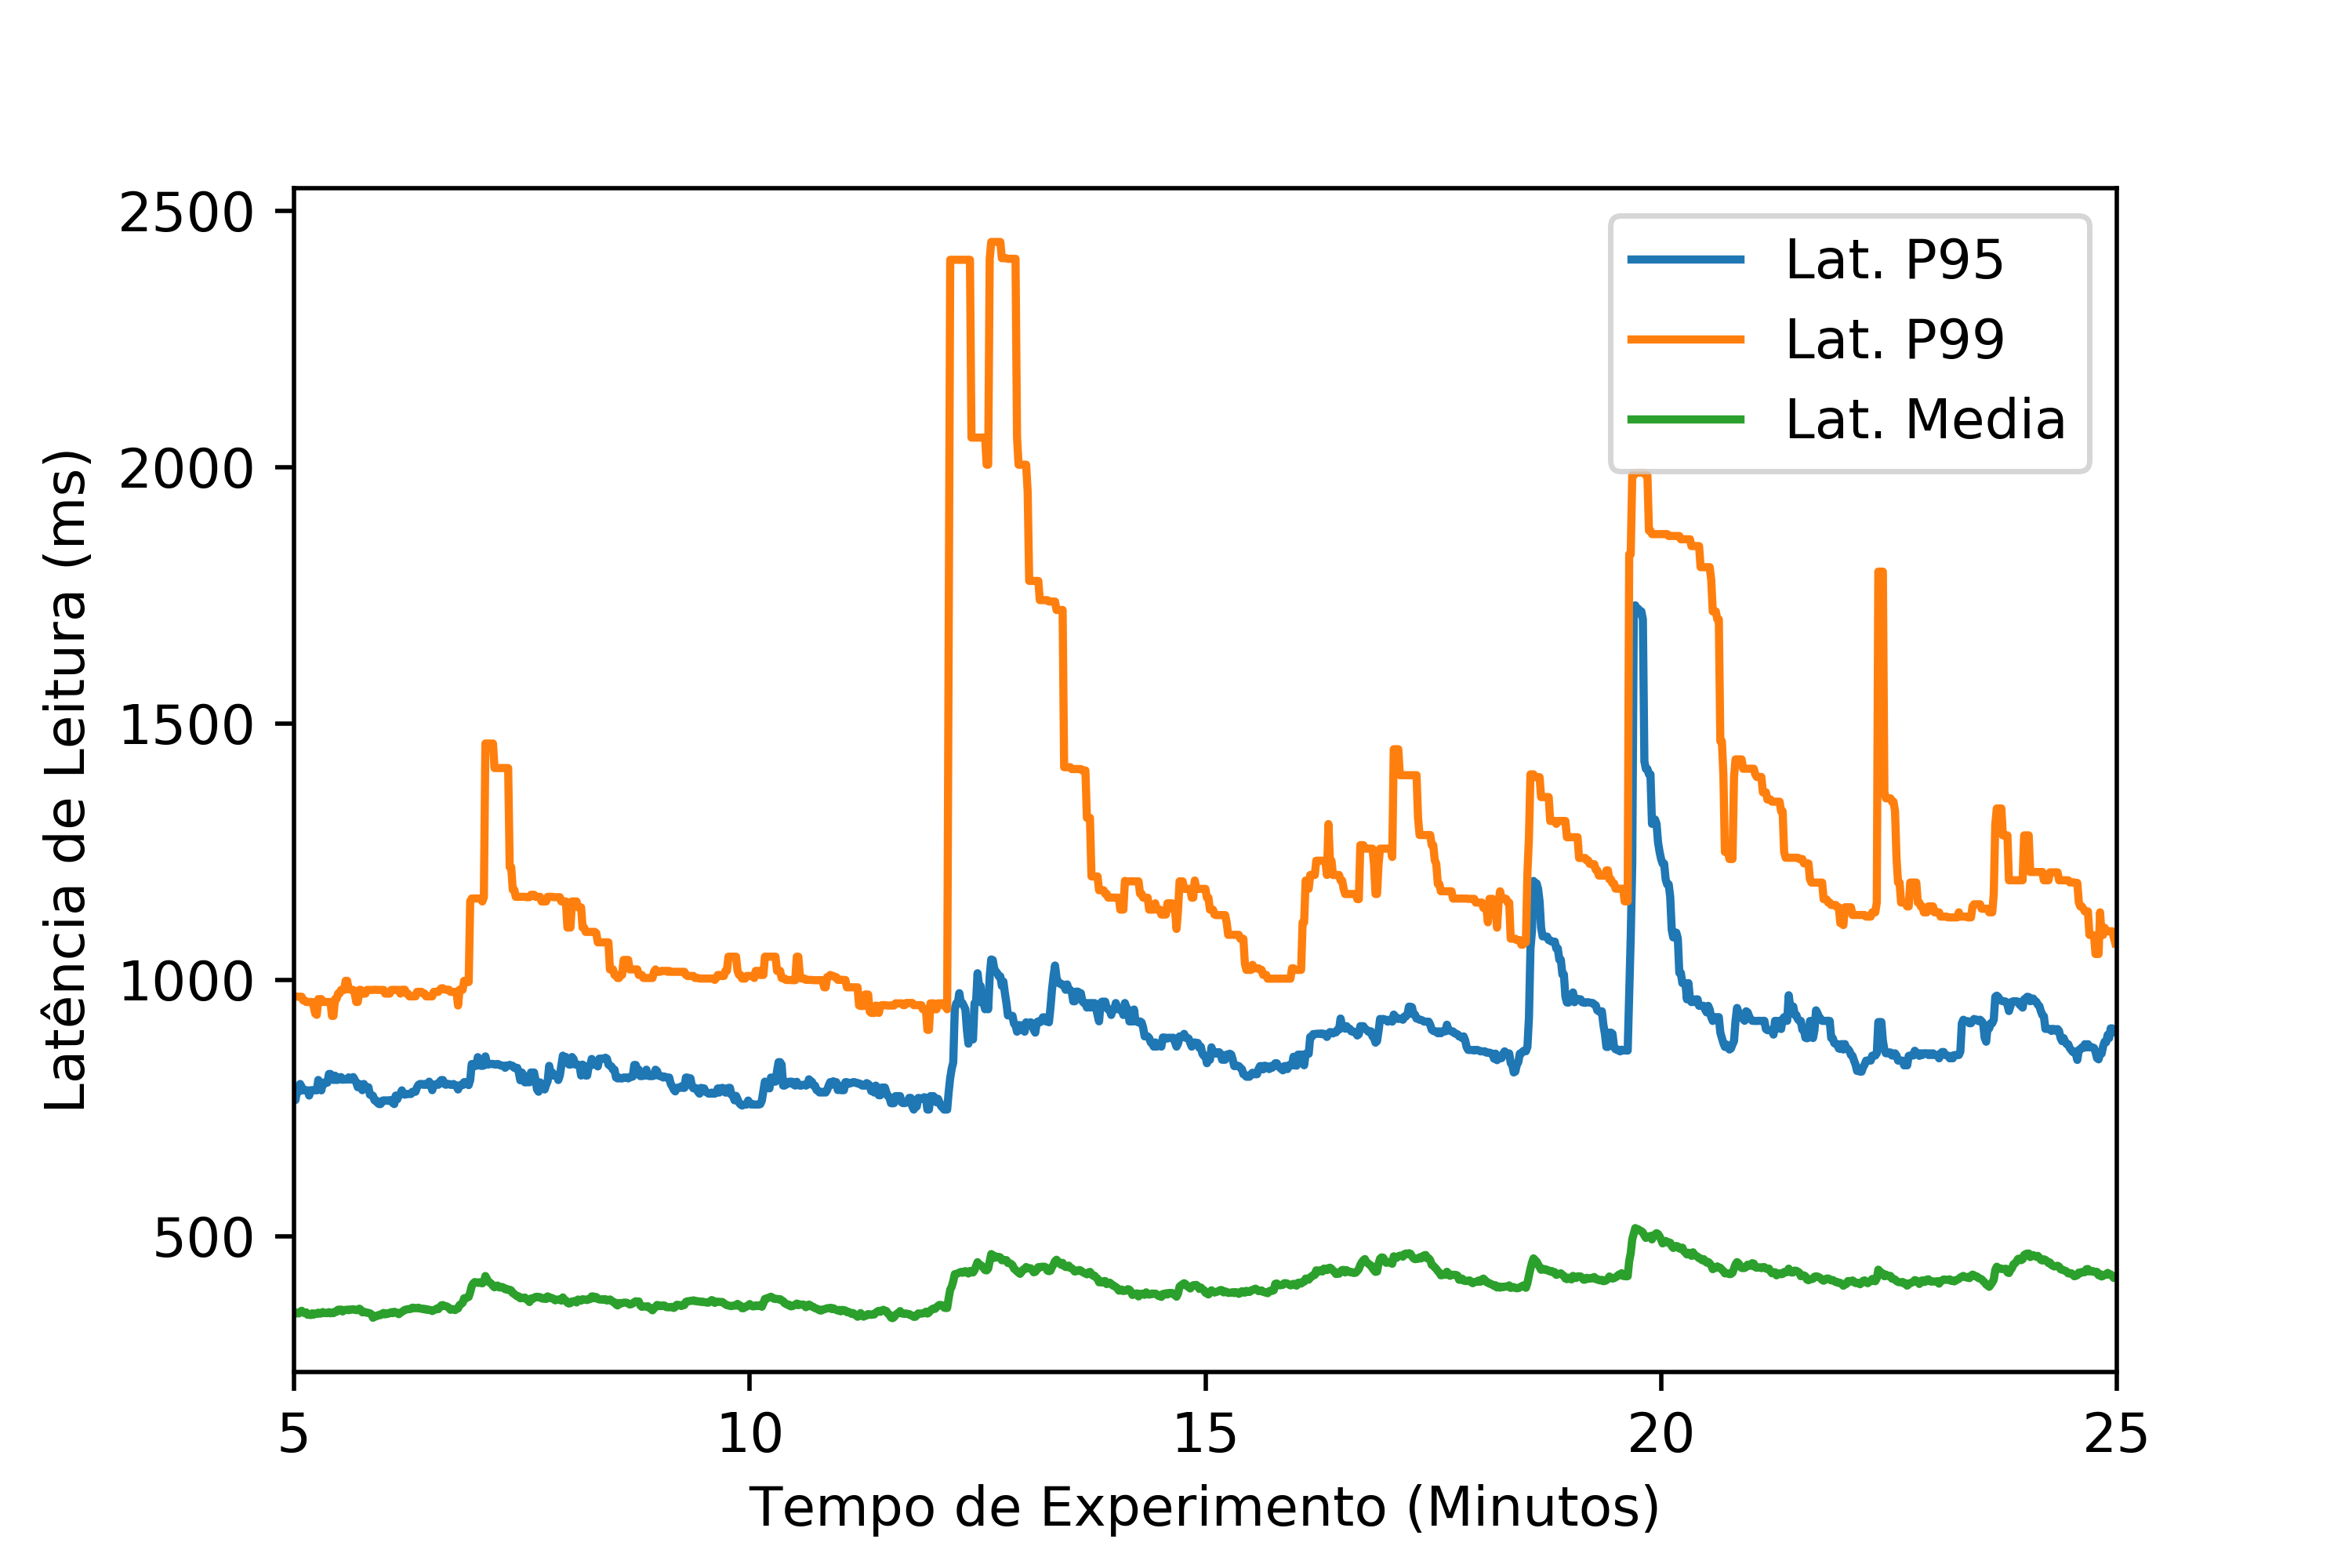
\includegraphics[scale=0.5]{img/pi3Read.png}
        \caption{Latências por segundo durante leitura no período de execução de 25m desconsiderando os 5m iniciais do simulador.}
        \label{fig:read}
    \end{figure}
}

\frame{
    \frametitle{Experimento 2}
    \framesubtitle{RPS de leitura}
    \begin{figure}[!ht]
        \centering
        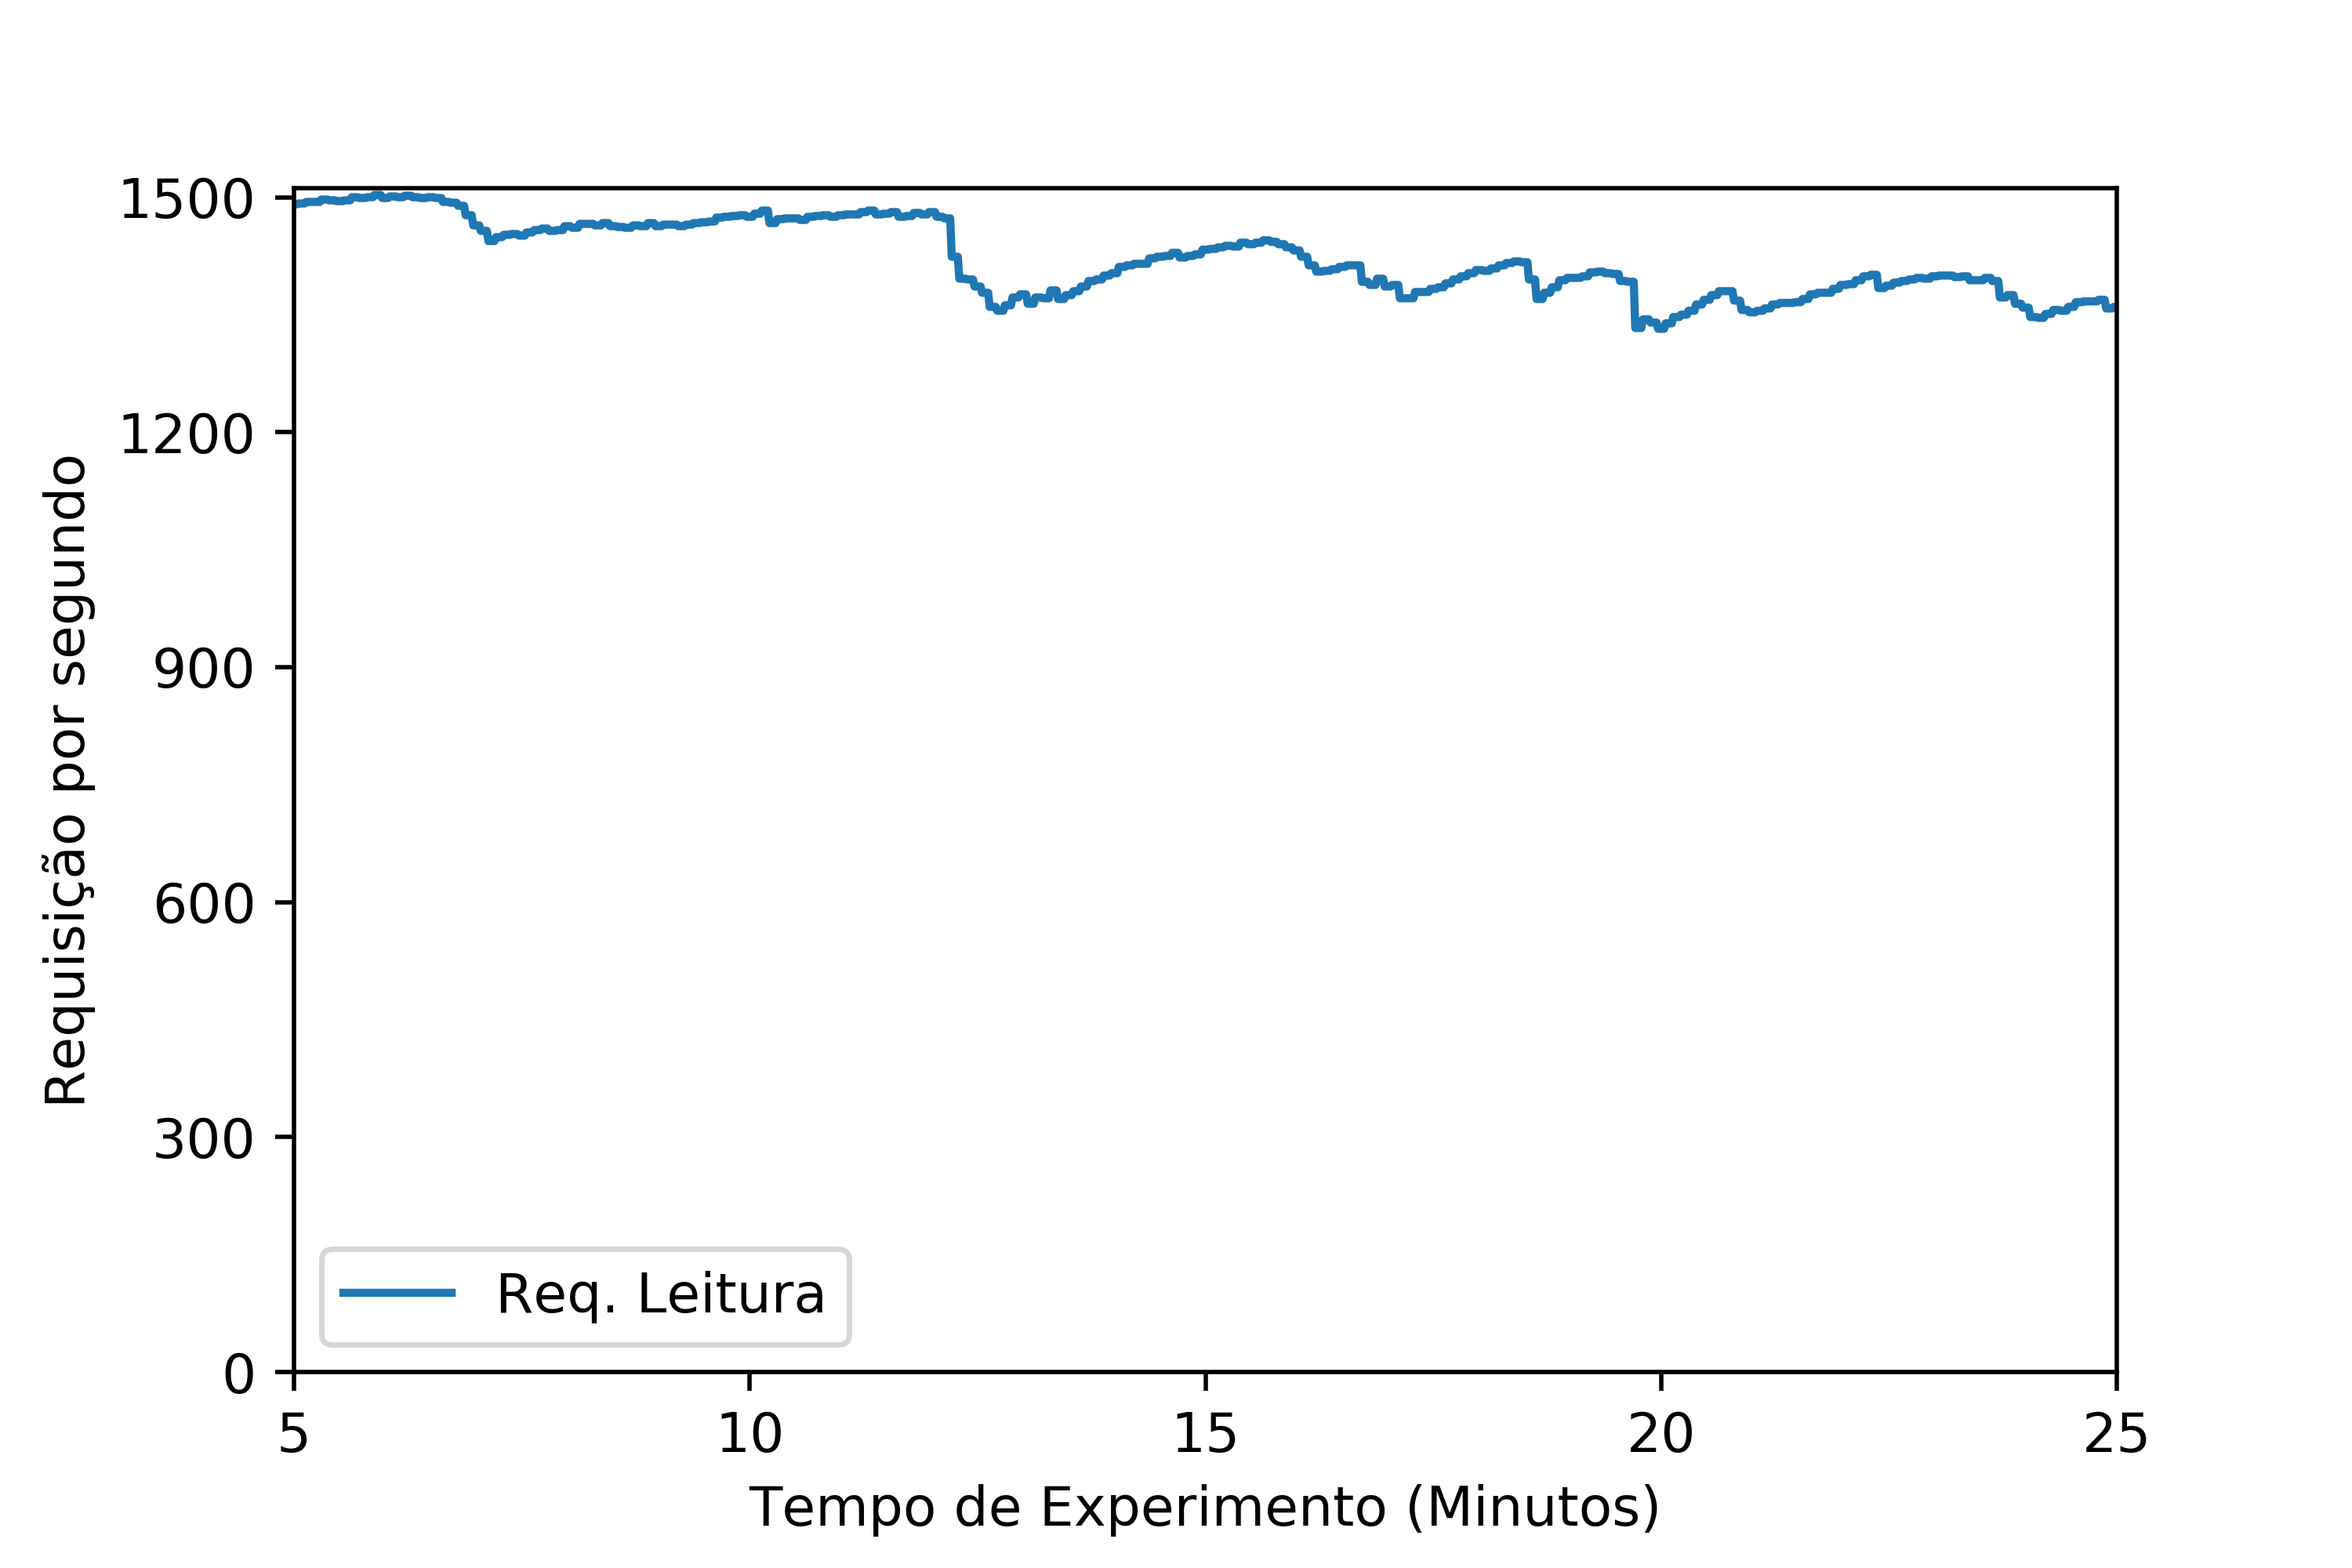
\includegraphics[scale=0.5]{img/pi3ReadRPS.png}
        \caption{Requisições por segundo durante leitura no período de execução de 25m desconsiderando os 5m iniciais do simulador.}
        \label{fig:readRPS}
    \end{figure}
}

\frame{
    \frametitle{Experimento 3}
    \framesubtitle{Latência de escrita}
    \begin{figure}[!ht]
        \centering
        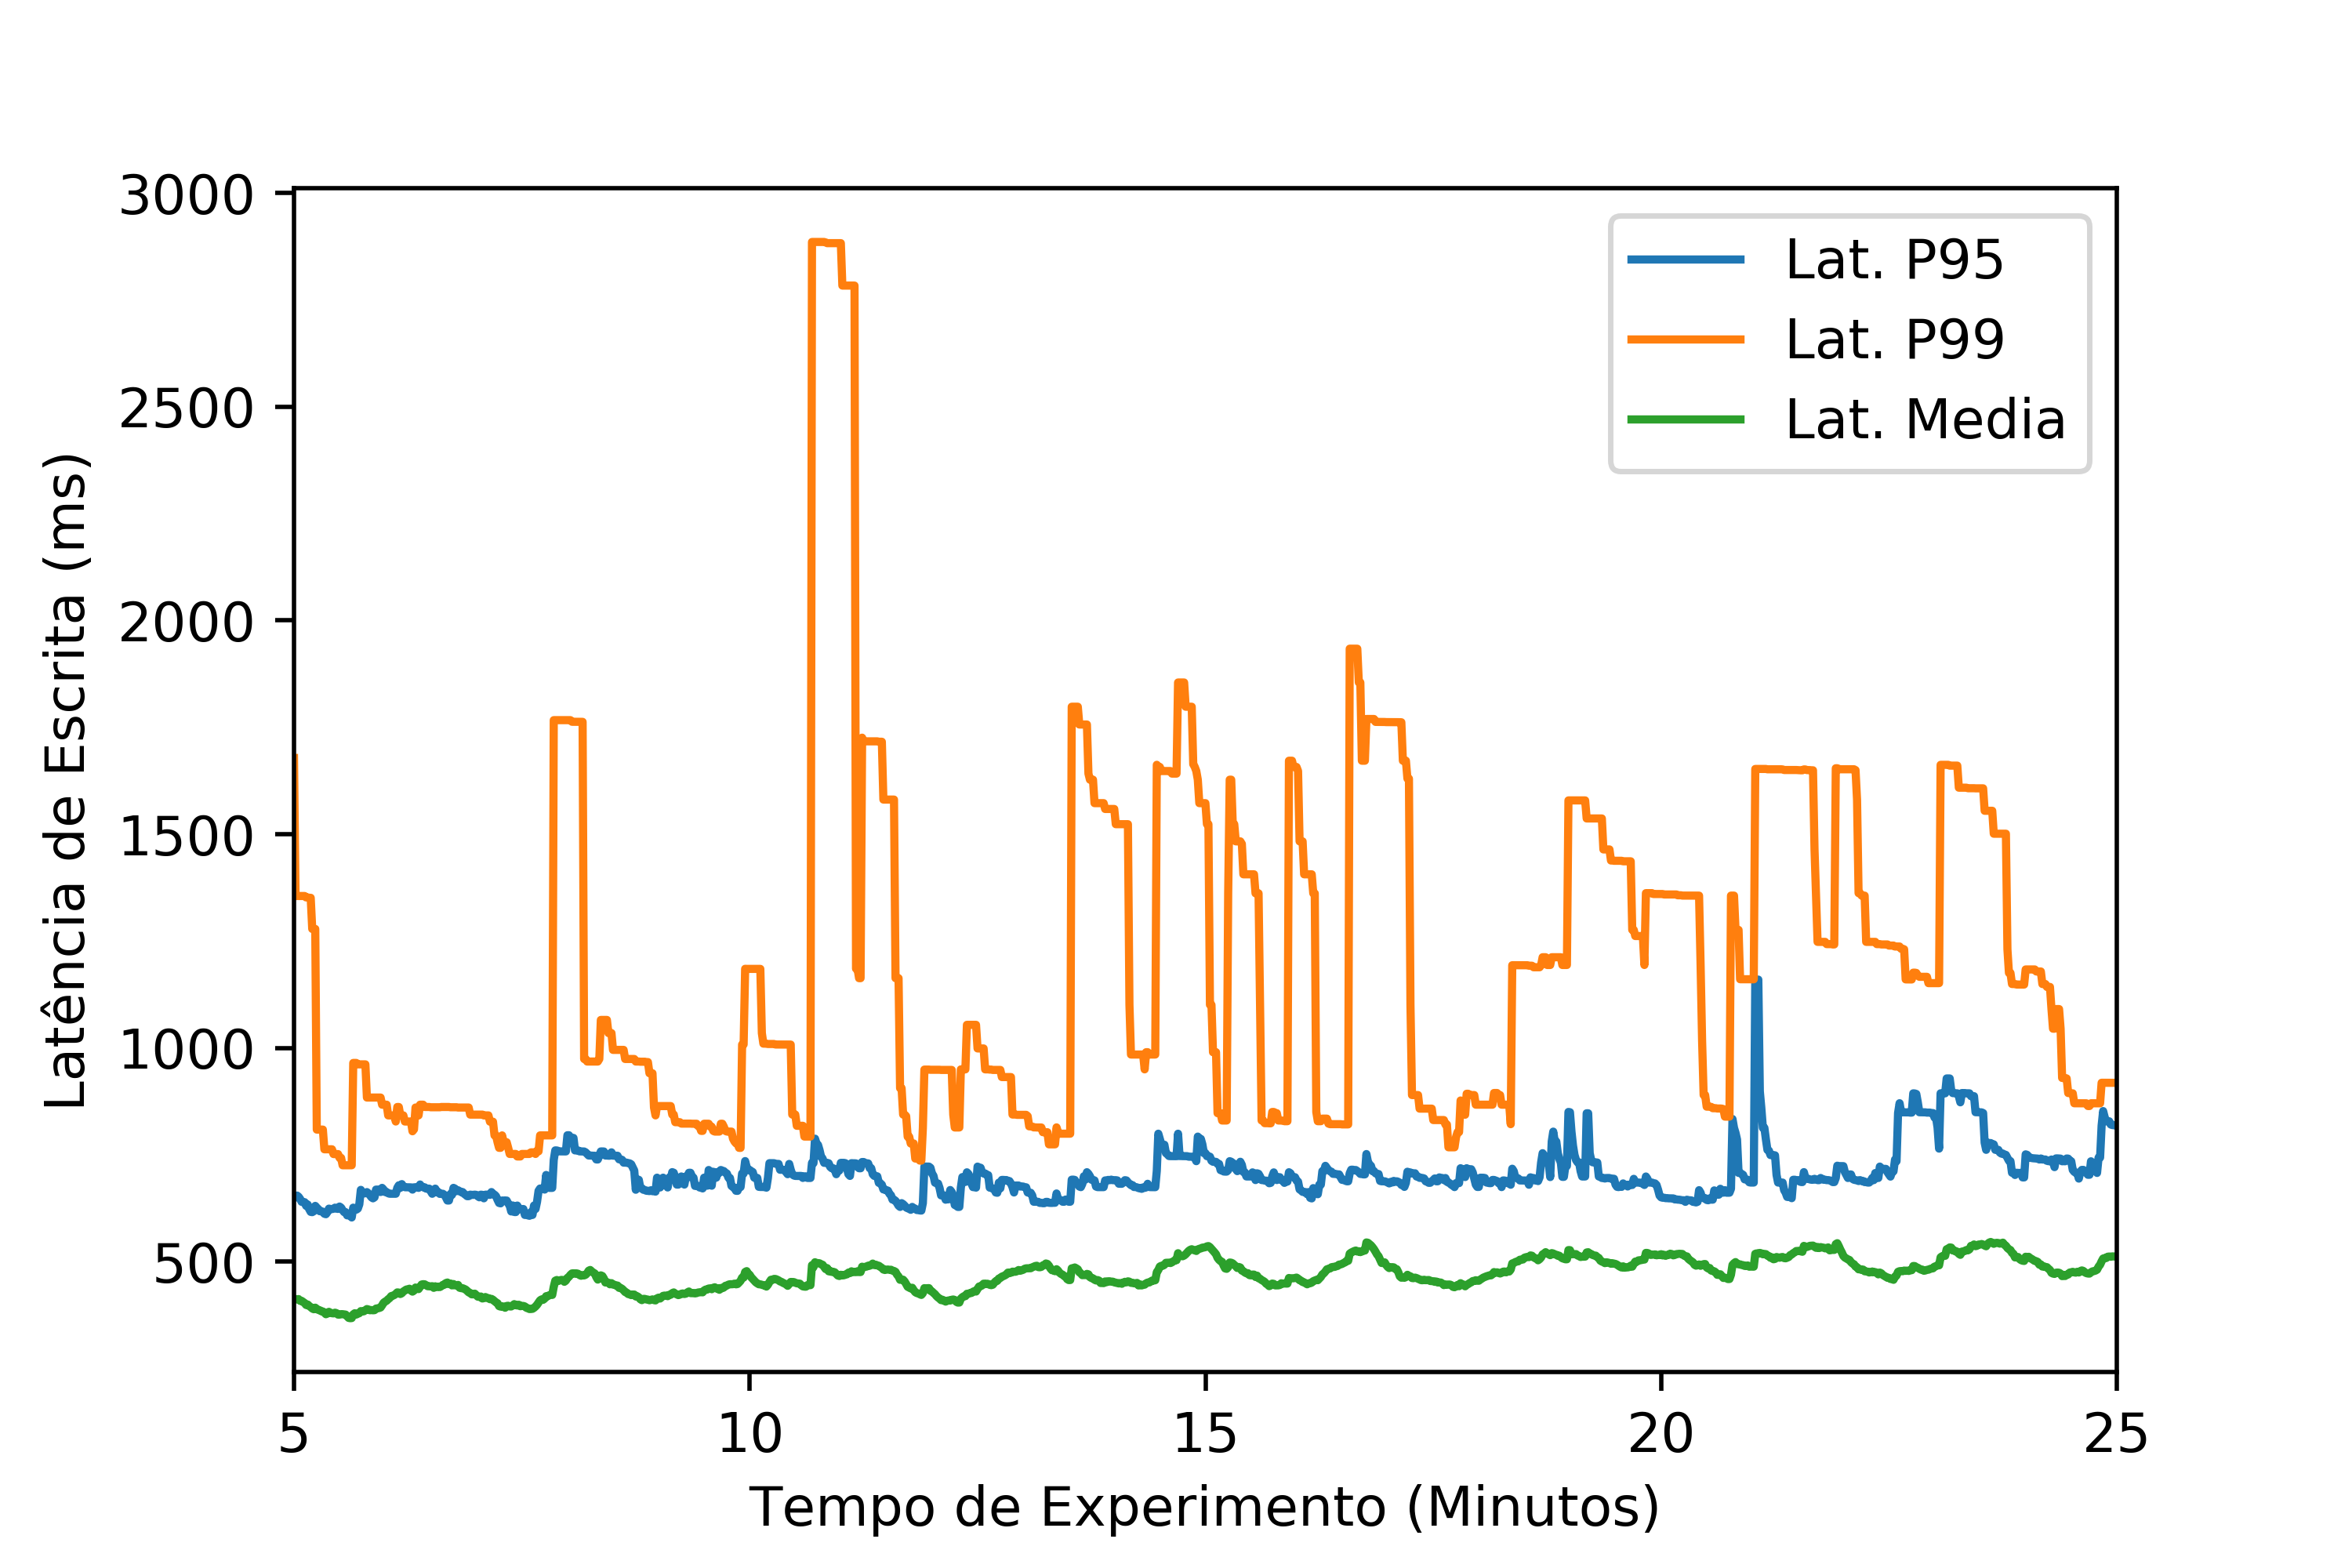
\includegraphics[scale=0.5]{img/pi3WriteInWriteAndRead.png}
        \caption{Latência por segundo durante escritas e leituras no período de execução de 25m desconsiderando os 5m iniciais do simulador.}
        \label{fig:readInWriteAndRead}
    \end{figure}
}

\frame{
    \frametitle{Experimento 3}
    \framesubtitle{Latência de leitura}
    \begin{figure}[!ht]
        \centering
        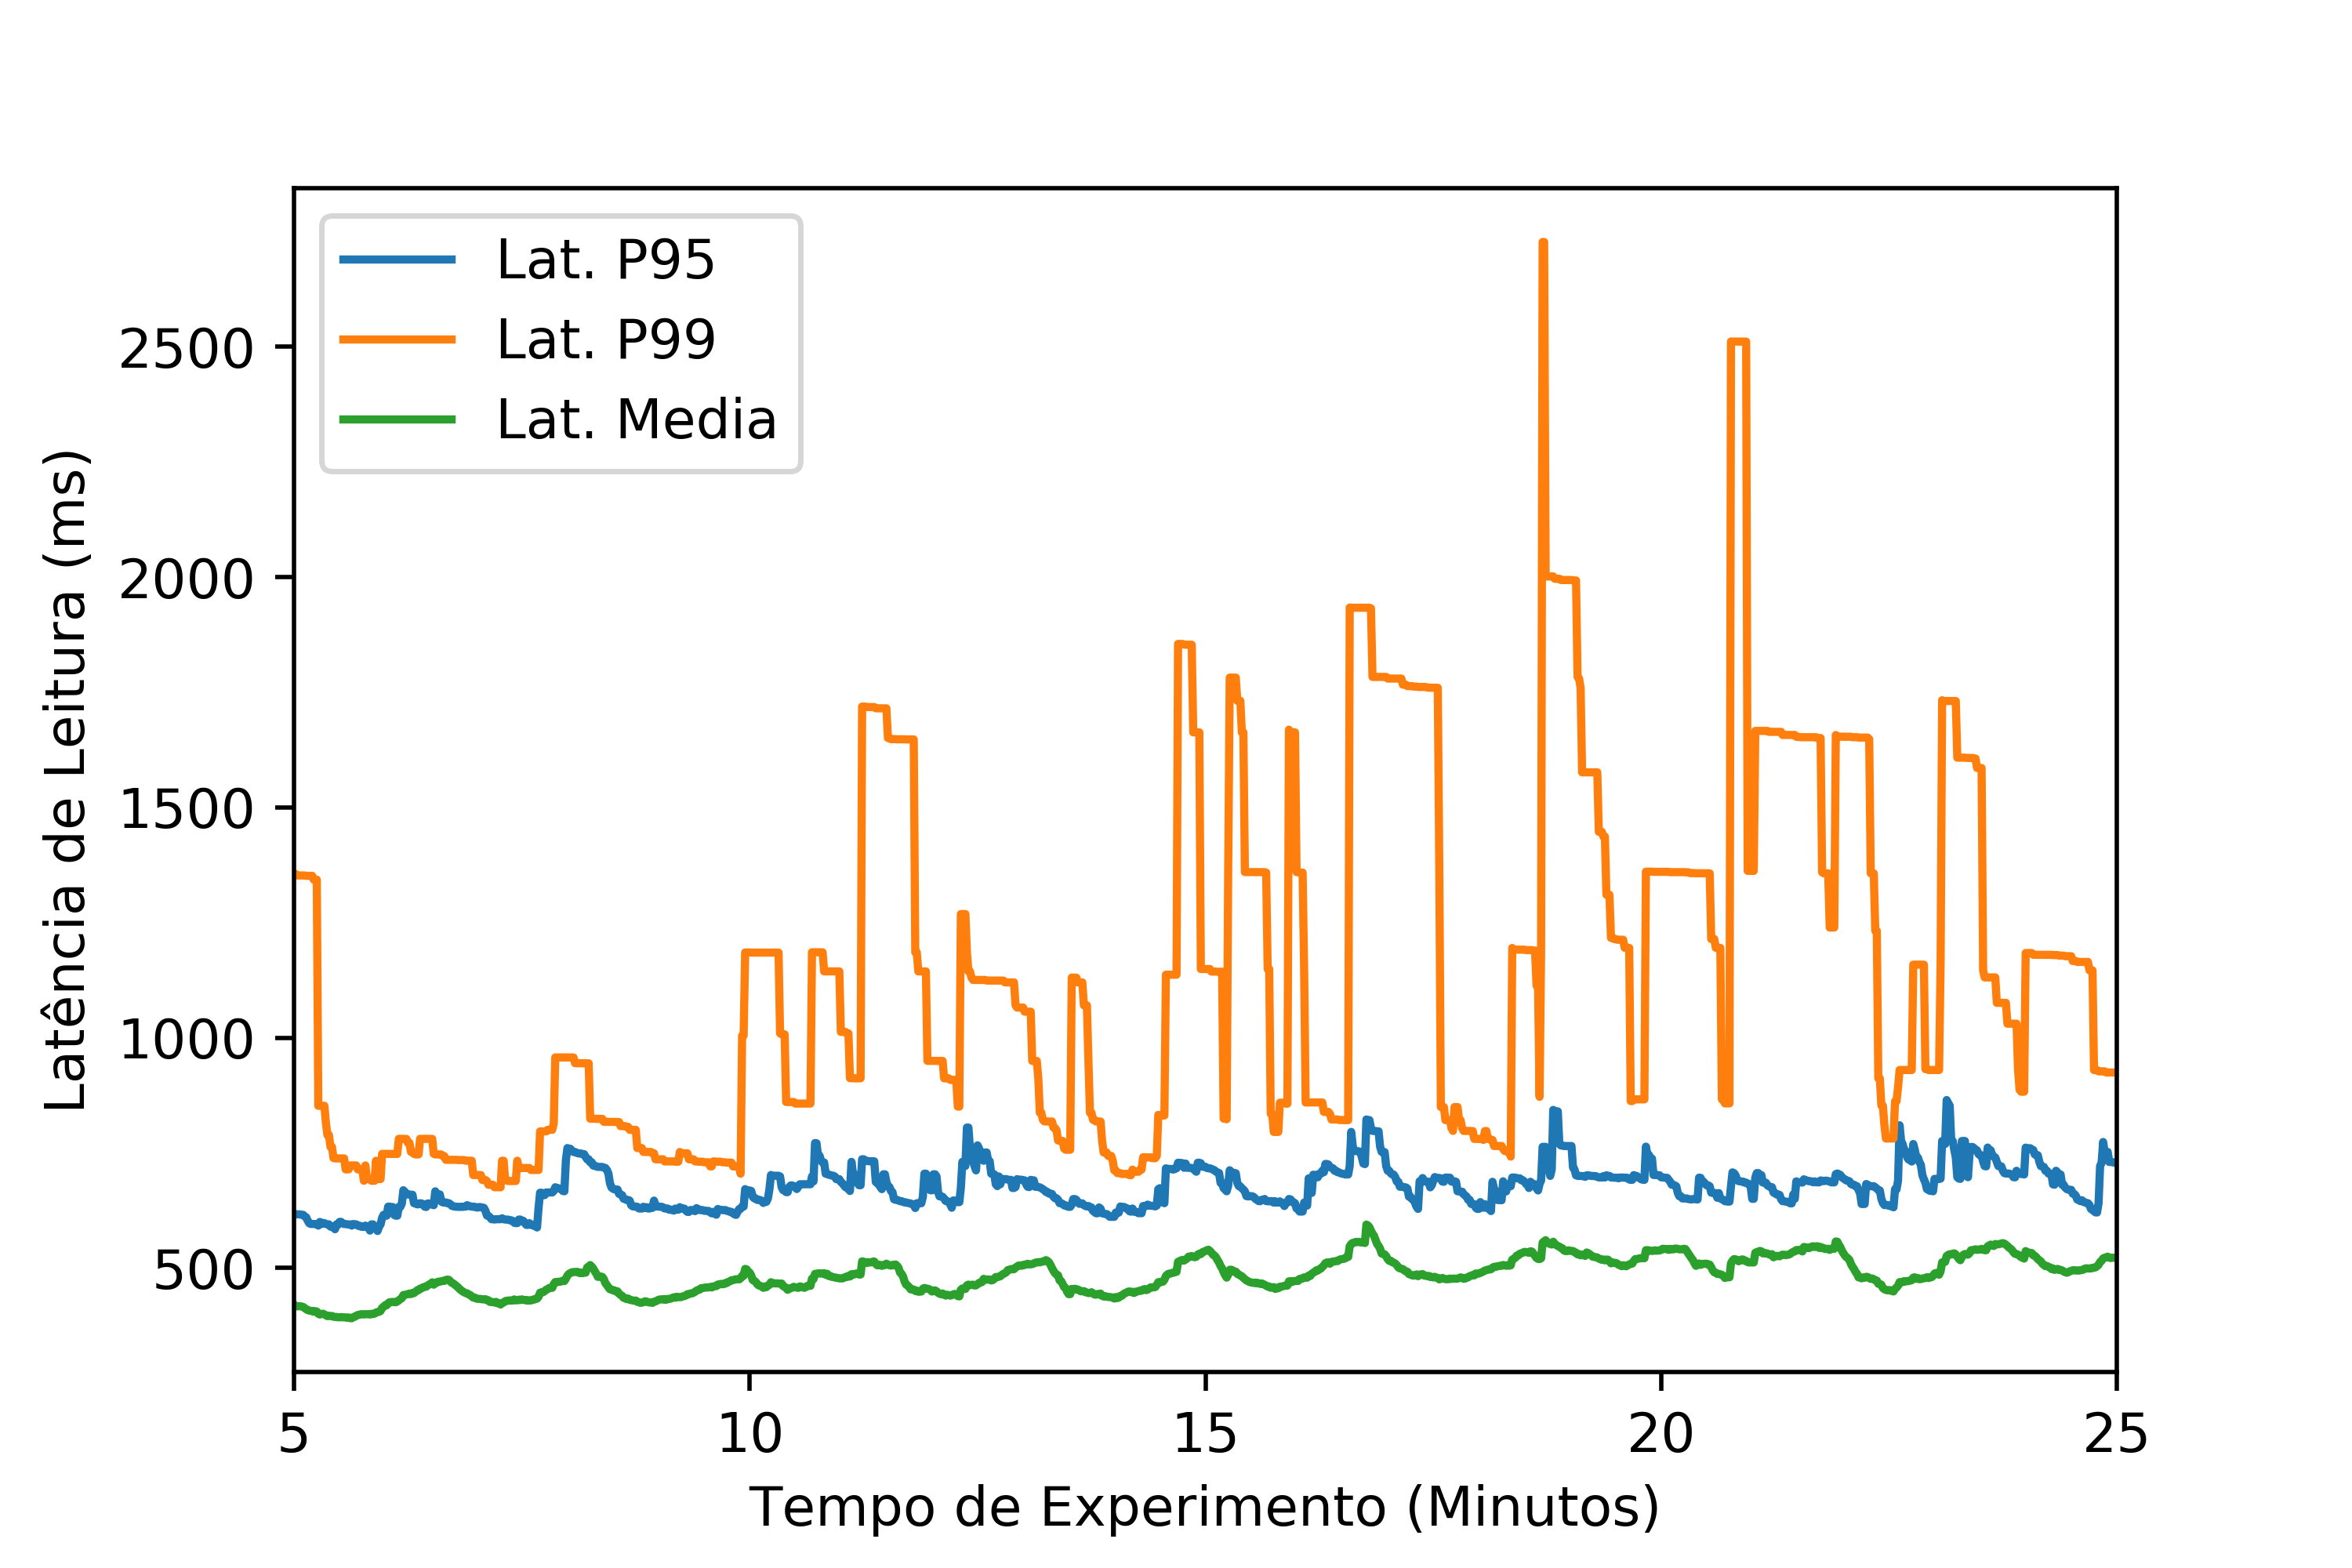
\includegraphics[scale=0.5]{img/pi3ReadInWriteAndRead.png}
        \caption{Latência por segundo durante escritas e leituras no período de execução de 25m desconsiderando os 5m iniciais do simulador.}
        \label{fig:writeInWriteAndRead}
    \end{figure}
}

\frame{
    \frametitle{Experimento 3}
    \framesubtitle{RPS de escrita e leitura}
    \begin{figure}[!ht]
        \centering
        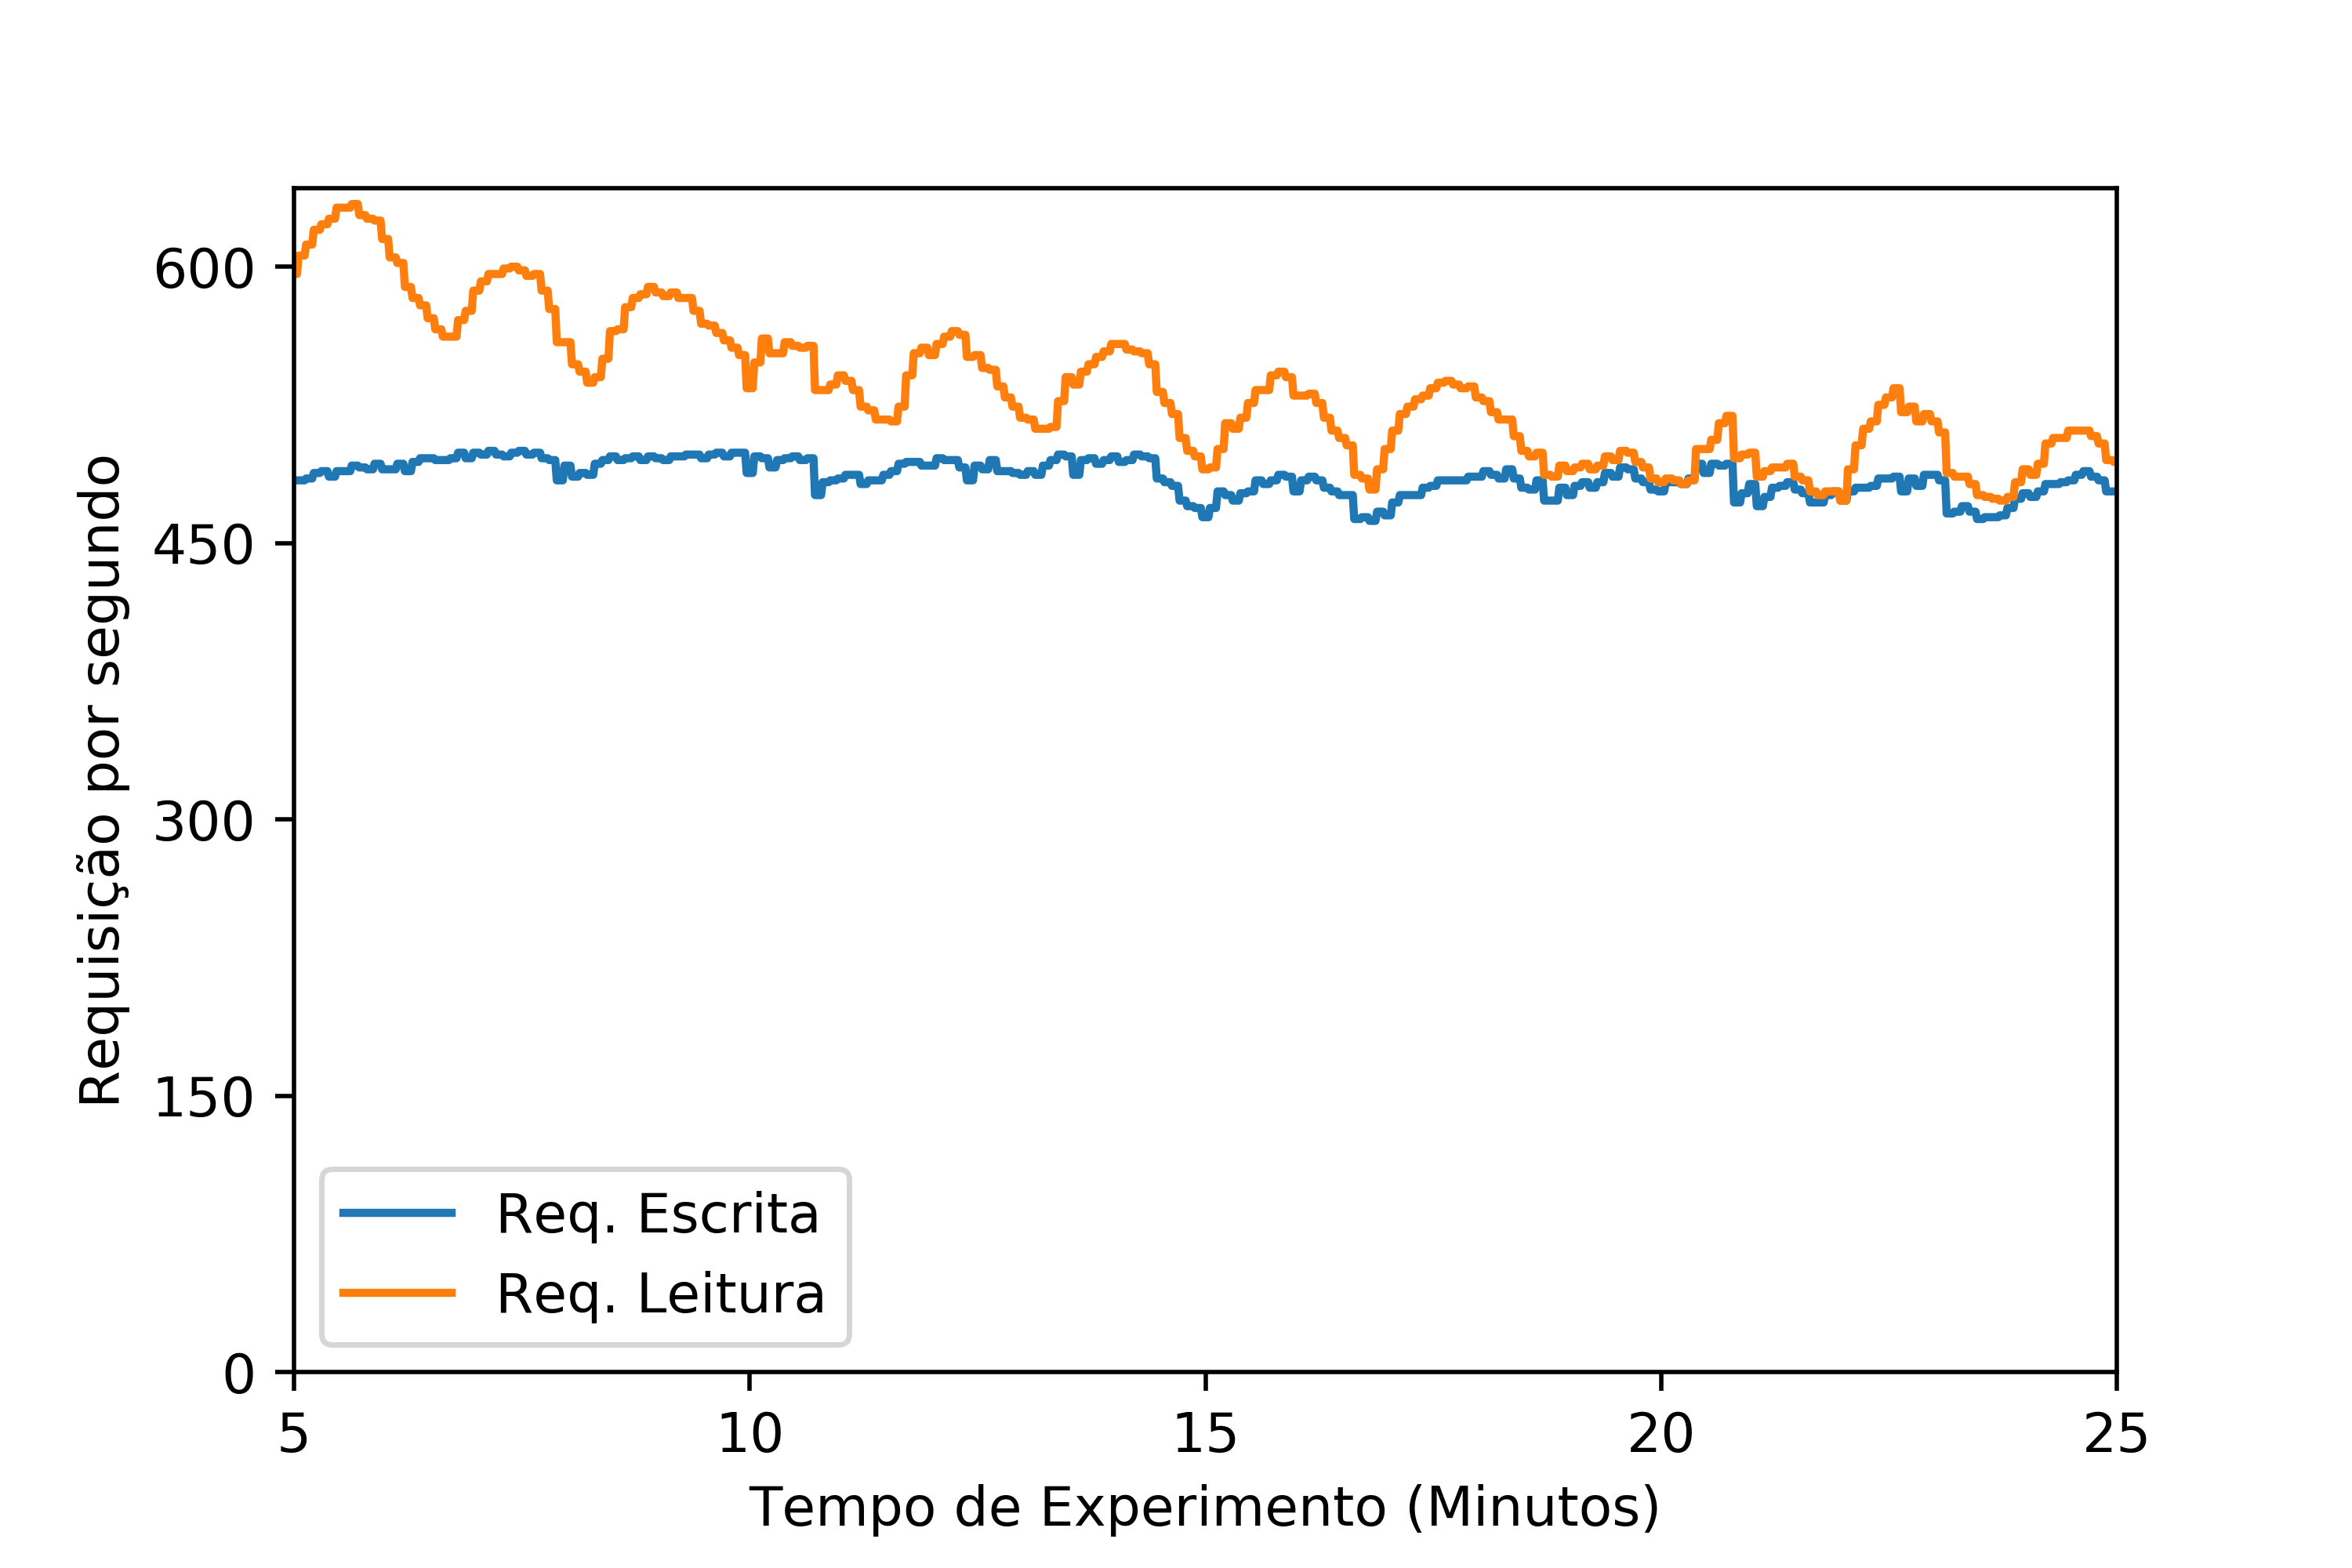
\includegraphics[scale=0.5]{img/pi3WriteAndReadRPS.png}
        \caption{Requisições por segundo durante escritas e leituras no período de execução de 25m desconsiderando os 5m iniciais do simulador.}
        \label{fig:readAndWriteRPS}
    \end{figure}
}

%============================================================================================
\section{Considerações Finais}
\frame{
  \frametitle{Considerações Finais}
  \begin{block}{ }
    \begin{itemize}
       \item Raspberry PI 3 apresentou-se eficiênte nos cenários propóstos, tanto em latência quanto em operações por segundo; 
       \item Latência em percentil 95 entre 500ms e 1000ms, enquanto a latência média se manteve abaixo de 500ms;
       \item Realizando em torno de 1.100 operações por segundo;
       \item Assim sendo, tais resultados demonstram a possibilidade de uso da \textit{smallboard} em aplicações que tenham necessidades semelhantes. 
    \end{itemize}
  \end{block}
}

\frame{
    \frametitle{Considerações Finais}
    \begin{block}{}
        \begin{itemize}
            \item Técnicas de \textit{tuning} não foram exploradas no trabalho aqui apresentado;
            \item Tudo utilizado na pesquisa encontra-se disponivel no Github para reprodução;
                \begin{itemize}
                    \item \url{github.com/SouzaGuilherme/research_PI3_evaluate_experiment};
                    \item \textit{scripts};
                    \item Resultados acompanhados do inicio do simulador.
                \end{itemize}
        \end{itemize}
    \end{block}
}

\frame{
  \frametitle{Trabalhos Futuros}
  \begin{block}{ }
    \begin{itemize}
       \item Simular cenários mais realisticos como os gerados pela própria \textit{Netflix} e \textit{Facebook}; 
       \item Estudo de aplicações mais restritas como as de industria 4.0 e as de cidades inteligentes; 
       \item Aumemento horizontal do dispositivo, assim possibilitando um \textit{clustes} de Raspberry PI;
       \item Estudo de eficiência e possibilidades com a sua descendente, à Raspberry PI4.
    \end{itemize}
  \end{block}
}
\frame{
  \frametitle{Considerações Finais}
  \begin{block}{Agradecimentos}
    \begin{itemize}
      \item Grupo de Pesquisa: LUPS
      \item Grupo de Pesquisa: InterSCity
%      \item Orgãos de fomento: UFPEL
      \item Universidade Federal de Pelotas
      \item Universidade Estadual de São Paulo
      \item CAPES
    \end{itemize}
  \end{block}
  \begin{block}{Contato:}
    \textbf{E-mail:} \texttt{gdsdsilva@inf.ufpel.edu.br}
  \end{block}
  \begin{block}{\centering Dúvidas?}\end{block}
}

%==================================================================================

\end{document}
%==================================================================================

% \bibitem{norman} E. H. Norman {\em Japan's emergence as a modern
%   state} 1940: International Secretariat, Institute of Pacific
%   Relations.
